\documentclass[11pt,a4paper,oneside]{report}             % Single-side
\usepackage[utf8]{inputenc}
\usepackage[T1]{fontenc}
%\documentclass[11pt,a4paper,twoside,openright]{report}  % Duplex

%\PassOptionsToPackage{chapternumber=Huordinal}{magyar.ldf}
\usepackage{amsmath}
\usepackage{amssymb}
\usepackage{enumerate}
\usepackage[thmmarks]{ntheorem}
\usepackage{graphics}
\usepackage{epsfig}
\usepackage{listings}
\usepackage{color}
%\usepackage{fancyhdr}
\usepackage{lastpage}
\usepackage{anysize}
\usepackage[magyar]{babel}
\usepackage{sectsty}
\usepackage{setspace}  % Ettol a tablazatok, abrak, labjegyzetek maradnak 1-es sorkozzel!
\usepackage[hang]{caption}
\usepackage{hyperref}

%--------------------------------------------------------------------------------------
% Main variables
%--------------------------------------------------------------------------------------
\newcommand{\vikszerzo}{Mózes Ádám István}
\newcommand{\vikkonzulens}{dr.~Félegyházi Márk}
\newcommand{\vikcim}{Elektronikus terelõk}
\newcommand{\viktanszek}{Hálózati Rendszerek és Szolgáltatások Tanszék}
\newcommand{\vikdoktipus}{Szakdolgozat}
\newcommand{\vikdepartmentr}{Bódis-Szomorú András}

%--------------------------------------------------------------------------------------
% Page layout setup
%--------------------------------------------------------------------------------------
% we need to redefine the pagestyle plain
% another possibility is to use the body of this command without \fancypagestyle
% and use \pagestyle{fancy} but in that case the special pages
% (like the ToC, the References, and the Chapter pages)remain in plane style

\pagestyle{plain}
%\setlength{\parindent}{0pt} % áttekinthetõbb, angol nyelvû dokumentumokban jellemzõ
%\setlength{\parskip}{8pt plus 3pt minus 3pt} % áttekinthetõbb, angol nyelvû dokumentumokban jellemzõ
\setlength{\parindent}{12pt} % magyar nyelvû dokumentumokban jellemzõ
\setlength{\parskip}{0pt}    % magyar nyelvû dokumentumokban jellemzõ

\marginsize{35mm}{25mm}{15mm}{15mm} % anysize package
\setcounter{secnumdepth}{0}
\sectionfont{\large\upshape\bfseries}
\setcounter{secnumdepth}{2}
\singlespacing
\frenchspacing

%--------------------------------------------------------------------------------------
%	Setup hyperref package
%--------------------------------------------------------------------------------------
\hypersetup{
    bookmarks=true,            % show bookmarks bar?
    unicode=false,             % non-Latin characters in Acrobat’s bookmarks
    pdftitle={\vikcim},        % title
    pdfauthor={\vikszerzo},    % author
    pdfsubject={\vikdoktipus}, % subject of the document
    pdfcreator={\vikszerzo},   % creator of the document
    pdfproducer={Producer},    % producer of the document
    pdfkeywords={keywords},    % list of keywords
    pdfnewwindow=true,         % links in new window
    colorlinks=true,           % false: boxed links; true: colored links
    linkcolor=black,           % color of internal links
    citecolor=black,           % color of links to bibliography
    filecolor=black,           % color of file links
    urlcolor=black             % color of external links
}

%--------------------------------------------------------------------------------------
% Set up listings
%--------------------------------------------------------------------------------------
\lstset{
	basicstyle=\scriptsize\ttfamily, % print whole listing small
	keywordstyle=\color{black}\bfseries\underbar, % underlined bold black keywords
	identifierstyle=, 					% nothing happens
	commentstyle=\color{white}, % white comments
	stringstyle=\scriptsize\sffamily, 			% typewriter type for strings
	showstringspaces=false,     % no special string spaces
	aboveskip=3pt,
	belowskip=3pt,
	columns=fixed,
	backgroundcolor=\color{lightgray},
} 		
\def\lstlistingname{lista}	

%--------------------------------------------------------------------------------------
%	Some new commands and declarations
%--------------------------------------------------------------------------------------
\newcommand{\code}[1]{{\upshape\ttfamily\scriptsize\indent #1}}

% define references
\newcommand{\figref}[1]{\ref{fig:#1}.}
\renewcommand{\eqref}[1]{(\ref{eq:#1})}
\newcommand{\listref}[1]{\ref{listing:#1}.}
\newcommand{\sectref}[1]{\ref{sect:#1}}
\newcommand{\tabref}[1]{\ref{tab:#1}.}

\DeclareMathOperator*{\argmax}{arg\,max}
%\DeclareMathOperator*[1]{\floor}{arg\,max}
\DeclareMathOperator{\sign}{sgn}
\DeclareMathOperator{\rot}{rot}
\definecolor{lightgray}{rgb}{0.95,0.95,0.95}

\author{\vikszerzo}
\title{\viktitle}
\includeonly{
	abstract,
	acknowledgement,
	appendices,
	background,
	chapter3,
	declaration,
	futureimprovements,
	guideline,
	introduction,
	project,
	summary,
	titlepage,
}
%--------------------------------------------------------------------------------------
%	Setup captions
%--------------------------------------------------------------------------------------
\captionsetup[figure]{
%labelsep=none,
%font={footnotesize,it},
%justification=justified,
width=.75\textwidth,
aboveskip=10pt}

\renewcommand{\captionlabelfont}{\small\bf}
\renewcommand{\captionfont}{\footnotesize\it}

%--------------------------------------------------------------------------------------
% Table of contents and the main text
%--------------------------------------------------------------------------------------
\begin{document}
\singlespacing
%--------------------------------------------------------------------------------------
% Rovid formai es tartalmi tajekoztato
%--------------------------------------------------------------------------------------

\footnotesize
\begin{center}
\large
\textbf{\Large Általános információk, a diplomaterv szerkezete}\\
\end{center}

A diplomaterv szerkezete a BME Villamosmérnöki és Informatikai Karán:
\begin{enumerate}
\item	Diplomaterv feladatkiírás
\item	Címoldal
\item	Tartalomjegyzék
\item	A diplomatervezõ nyilatkozata az önálló munkáról és az elektronikus adatok kezelésérõl
\item	Tartalmi összefoglaló magyarul és angolul
\item	Bevezetés: a feladat értelmezése, a tervezés célja, a feladat indokoltsága, a diplomaterv felépítésének rövid összefoglalása
\item	A feladatkiírás pontosítása és részletes elemzése
\item	Elõzmények (irodalomkutatás, hasonló alkotások), az ezekbõl levonható következtetések
\item	A tervezés részletes leírása, a döntési lehetõségek értékelése és a választott megoldások indoklása
\item	A megtervezett mûszaki alkotás értékelése, kritikai elemzése, továbbfejlesztési lehetõségek
\item	Esetleges köszönetnyilvánítások
\item	Részletes és pontos irodalomjegyzék
\item	Függelék(ek)
\end{enumerate}

Felhasználható a következõ oldaltól kezdõdõ \LaTeX-Diplomaterv sablon dokumentum tartalma. 

A diplomaterv szabványos méretû A4-es lapokra kerüljön. Az oldalak tükörmargóval készüljenek (mindenhol 2.5cm, baloldalon 1cm-es kötéssel). Az alapértelmezett betûkészlet a 12 pontos Times New Roman, másfeles sorközzel.

Minden oldalon - az elsõ négy szerkezeti elem kivételével - szerepelnie kell az oldalszámnak.

A fejezeteket decimális beosztással kell ellátni. Az ábrákat a megfelelõ helyre be kell illeszteni, fejezetenként decimális számmal és kifejezõ címmel kell ellátni. A fejezeteket decimális aláosztással számozzuk, maximálisan 3 aláosztás mélységben (pl. 2.3.4.1.). Az ábrákat, táblázatokat és képleteket célszerû fejezetenként külön számozni (pl. 2.4. ábra, 4.2 táblázat vagy képletnél (3.2)). A fejezetcímeket igazítsuk balra, a normál szövegnél viszont használjunk sorkiegyenlítést. Az ábrákat, táblázatokat és a hozzájuk tartozó címet igazítsuk középre. A cím a jelölt rész alatt helyezkedjen el.

A képeket lehetõleg rajzoló programmal készítsék el, az egyenleteket egyenlet-szerkesztõ segítségével írják le (A \LaTeX~ehhez kézenfekvõ megoldásokat nyújt).

Az irodalomjegyzék szövegközi hivatkozása történhet a Harvard-rendszerben (a szerzõ és az évszám megadásával) vagy sorszámozva. A teljes lista névsor szerinti sorrendben a szöveg végén szerepeljen (sorszámozott irodalmi hivatkozások esetén hivatkozási sorrendben). A szakirodalmi források címeit azonban mindig az eredeti nyelven kell megadni, esetleg zárójelben a fordítással. A listában szereplõ valamennyi publikációra hivatkozni kell a szövegben (a \LaTeX-sablon a Bib\TeX~segítségével mindezt automatikusan kezeli). Minden publikáció a szerzõk után a következõ adatok szerepelnek: folyóirat cikkeknél a pontos cím, a folyóirat címe, évfolyam, szám, oldalszám tól-ig. A folyóirat címeket csak akkor rövidítsük, ha azok nagyon közismertek vagy nagyon hosszúak. Internet hivatkozások megadásakor fontos, hogy az elérési út elõtt megadjuk az oldal tulajdonosát és tartalmát (mivel a link egy idõ után akár elérhetetlenné is válhat), valamint az elérés idõpontját.

\vspace{5mm}
Fontos:
\begin{itemize}
	\item A szakdolgozat készítõ / diplomatervezõ nyilatkozata (a jelen sablonban szereplõ szövegtartalommal) kötelezõ elõírás Karunkon ennek hiányában a szakdolgozat/diplomaterv nem bírálható és nem védhetõ !
	\item Mind a dolgozat, mind a melléklet maximálisan 15 MB méretû lehet !
\end{itemize}

\vspace{5mm}
\begin{center}
Jó munkát, sikeres szakdolgozat készítést ill. diplomatervezést kívánunk !
\end{center}

\normalsize

%--------------------------------------------------------------------------------------
% Feladatkiiras (a tanszeken atveheto, kinyomtatott valtozat)
%--------------------------------------------------------------------------------------
\clearpage
\begin{center}
\large
\textbf{FELADATKI�R�S}\\
\end{center}

A feladatki�r�st a tansz�ki adminisztr�ci�ban lehet �tvenni, �s a leadott munk�ba eredeti, tansz�ki pecs�ttel ell�tott �s a tansz�kvezet� �ltal al��rt lapot kell belef�zni (ezen oldal \emph{helyett}, ez az oldal csak �tmutat�s). Az elektronikusan felt�lt�tt dolgozatban m�r nem kell beleszerkeszteni ezt a feladatki�r�st.





\pagenumbering{arabic}
\onehalfspacing
%--------------------------------------------------------------------------------------
%	The title page
%--------------------------------------------------------------------------------------
\begin{titlepage}
    \begin{center}
        
\includegraphics[width=60mm,keepaspectratio]{figures/BMElogo.png}\\
        \vspace{0.3cm}
        \textbf{Budapesti Mûszaki és Gazdaságtudományi Egyetem}\\
        \textmd{Villamosmérnöki és Informatikai Kar}\\
        \textmd{\viktanszek}\\[5cm]

        \vspace{0.4cm}
        {\huge \bfseries \vikcim}\\[0.8cm]
        \vspace{0.5cm}
        \textsc{\Large \vikdoktipus}\\[4cm]

        \begin{tabular}{cc}
            \makebox[7cm]{\emph{Készítette}} & \makebox[7cm]{\emph{Konzulens}} \\
            \makebox[7cm]{\vikszerzo} & \makebox[7cm]{\vikkonzulens} \\
            \makebox[7cm]{} & \makebox[7cm]{\vikkulsokonzulens}
        \end{tabular}

        \vfill
        {\large \today}
    \end{center}
\end{titlepage}

\tableofcontents\vfill
%--------------------------------------------------------------------------------------
% Nyilatkozat
%--------------------------------------------------------------------------------------
\begin{center}
\large
\textbf{HALLGATÓI NYILATKOZAT}\\
\end{center}

Alulírott \emph{\vikszerzo}, szigorló hallgató kijelentem, hogy ezt a szakdolgozatot meg nem engedett segítség nélkül, saját magam készítettem, csak a megadott forrásokat (szakirodalom, eszközök stb.) használtam fel. Minden olyan részt, melyet szó szerint, vagy azonos értelemben, de átfogalmazva más forrásból átvettem, egyértelmûen, a forrás megadásával megjelöltem.

Hozzájárulok, hogy a jelen munkám alapadatait (szerzõ(k), cím, angol és magyar nyelvû tartalmi kivonat, készítés éve, konzulens(ek) neve) a BME VIK nyilvánosan hozzáférhetõ elektronikus formában, a munka teljes szövegét pedig az egyetem belsõ hálózatán keresztül (vagy autentikált felhasználók számára) közzétegye. Kijelentem, hogy a benyújtott munka és annak elektronikus verziója megegyezik. Dékáni engedéllyel titkosított diplomatervek esetén a dolgozat szövege csak 3 év eltelte után válik hozzáférhetõvé.

\begin{flushleft}
\vspace*{1cm}
Budapest, \today
\end{flushleft}

\begin{flushright}
 \vspace*{1cm}
 \makebox[7cm]{\rule{6cm}{.4pt}}\\
 \makebox[7cm]{\emph{\vikszerzo}}\\
 \makebox[7cm]{hallgató}
\end{flushright}
\thispagestyle{empty}

\vfill
\clearpage
\thispagestyle{empty} % an empty page

%----------------------------------------------------------------------------
% Abstract in hungarian
%----------------------------------------------------------------------------
\chapter*{Kivonat}\addcontentsline{toc}{chapter}{Kivonat}

Jelen dokumentum egy diplomaterv sablon, amely formai keretet ad a BME Villamosm�rn�ki �s Informatikai Kar�n v�gz� hallgat�k �ltal elk�sz�tend� szakdolgozatnak �s diplomatervnek. A sablon haszn�lata opcion�lis. Ez a sablon \LaTeX~alap�, a \emph{TeXLive} \TeX-implement�ci�val �s a PDF-\LaTeX~ford�t�val m�k�d�k�pes.
\vfill

%----------------------------------------------------------------------------
% Abstract in english
%----------------------------------------------------------------------------
\chapter*{Abstract}\addcontentsline{toc}{chapter}{Abstract}

This document is a \LaTeX-based skeleton for BSc/MSc~theses of students at the Electrical Engineering and Informatics Faculty, Budapest University of Technology and Economics. The usage of this skeleton is optional. It has been tested with the \emph{TeXLive} \TeX~implementation, and it requires the PDF-\LaTeX~compiler.
\vfill


%----------------------------------------------------------------------------
\chapter*{Bevezet�}\addcontentsline{toc}{chapter}{Bevezet�}
%----------------------------------------------------------------------------

A bevezet� tartalmazza a diplomaterv-ki�r�s elemz�s�t, t�rt�nelmi el�zm�nyeit, a feladat indokolts�g�t (a motiv�ci� le�r�s�t), az eddigi megold�sokat, �s ennek t�kr�ben a hallgat� megold�s�nak �sszefoglal�s�t.

A bevezet� szok�s szerint a diplomaterv fel�p�t�s�vel z�r�dik, azaz annak r�vid le�r�s�val, hogy melyik fejezet mivel foglalkozik.


\chapter{Háttérinformációk}

\section{Motiváció}
Ez a szekció betekintést enged mind a közösség által fejlesztett, mint a fizetős
\todo[inline]{okosabb nevet?} változat fejlesztése során felmerülő nehézségekbe, esetleges
anomáliákba.

\todo{Tünetek - okok kifejtése}

Időközben magasabb szintről is felmerült az igény, hogy legyünk tisztában

\section{Különböző megközelítések vizsgálata}

Az egyes megközelítések feltérképezéséhez és megvizsgálásához remek kiindulási alapot adott az
alábbi publikáció: \url{http://citeseerx.ist.psu.edu/viewdoc/download?doi=10.1.1.132.4843&rep=rep1&type=pdf}.

\subsection{Attack trees}

Az \emph{Attack trees} egy olyan módszer, amellyel egy adott támadást elemezhetünk egyszerűen, egy
faként reprezentálva az alábbi szabályok mentén:
\begin{enumerate}
    \item A fa gyökerében az az esemény áll, amely bekövetkezésekor a támadást sikeresnek tekintjük.
    \item A szülő és a gyerek eseménye között az a kapcsolat, hogy a szülő eseménye akkor, és 
        csak akkor következik be, ha a gyerek eseménye is.
        Összekapcsolt gyerekek esetén akkor és csak akkor, ha mindegyik gyerek eseménye bekövetkezett.
\end{enumerate}
Miután megtaláltuk az eseményeink függőségeit (pontosabban a további felbontásnak már nem lenne
értelme), lehetőségünk van ezeket különféle szempontokból elemezni, például az alábbi szempontok mentén:
\begin{itemize}
    \item Lehetséges-e egyáltalán az esemény bekövetkezése?
    \item Mekkora költséggel jár előidézni az eseményt?
    \item Mekkora költséggel jár megelőzni az eseményt?
    \item Szükséges-e különleges felszerelés az előidézéshez?
\end{itemize}

\missingfigure{Példa}

Az alábbi szempontok segíthetnek eldönteni, hogy megéri-e foglalkozni a védelem kialakításával,
szem előtt tartva, hogy mit feltételezünk a támadóról.

Habár a módszer kellően könnyedén értelmezhető (hiszen csupán egy fát használ) és könnyedén
alkalmazható, számunkra kevésbé használható, hiszen nem kellően széleskörű, és megoldásokat egyáltalán nem szolgáltat,
és a teljesség sem garantált.

\subsection{Abuse/Misuse cases}

Az \emph{Misuse cases} az ismert \emph{use case} diagramnak a kifordított változata, azaz ahelyett,
hogy azt modelleznénk, hogy egy adott szereplő milyen tevékenységeket végezhet el, itt inkább azt
modellezzük, hogy egy rosszindulatú szereplő milyen nemkívánt tevékenységeket végezne el, azaz
meghatározhatjuk azokat a tevékenységeket, amelyeket a \emph{rendszernek tiltania kellene}.

\begin{figure}[h]
    \centering
    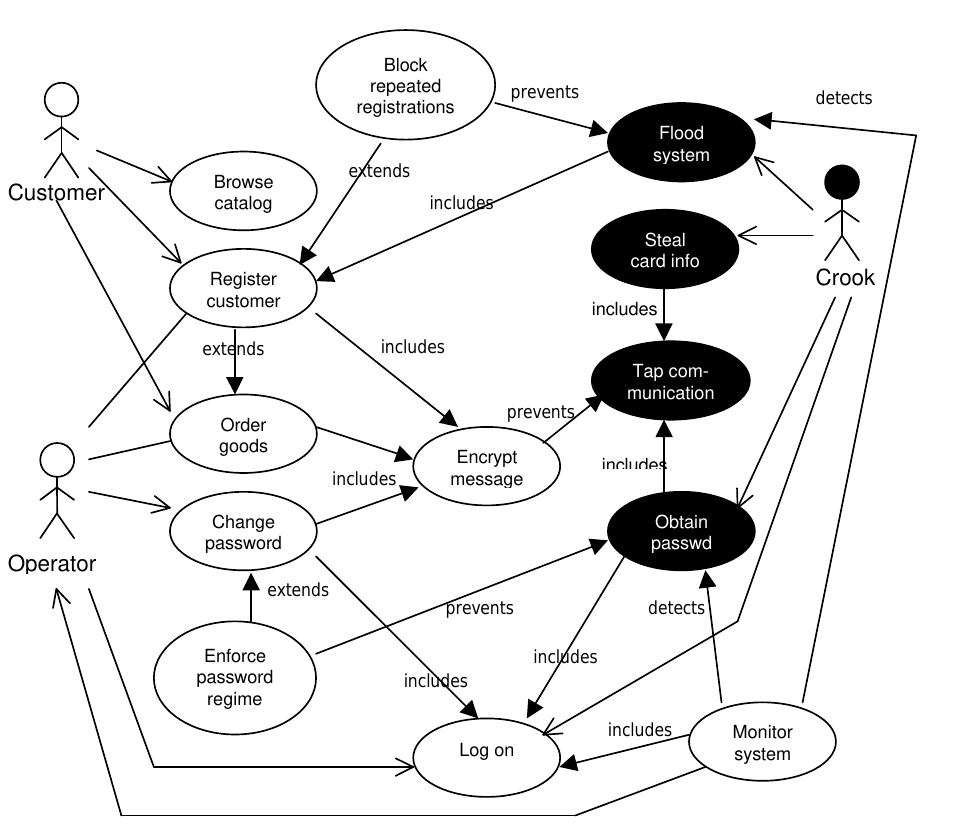
\includegraphics[width=\textwidth, height=0.25\textheight, keepaspectratio]{figures/misusecase.png}
\end{figure}

\FloatBarrier
\subsection{ISO 27000-as család}
\subsubsection{ISO 27001:2013}
Ellentétben a korábbi megközelítésekkel, az \emph{ISO 27001}-es szabvány 

Habár elsőre nem tűnik indokoltnak a megemlítése, elég csupán arra gondolnunk, hogy
egy termék fejlesztésekor elvárhatjuk, hogy a belső infrastruktúránk biztonságos.
Ahogy a cég (és ezzel együtt az infrastruktúra) növekszik, egyre inkább fontossá
válik egy olyan kész keret bevezetése, amelyet felhasználva biztonságosabb rendszert építhetünk.

\subsection{Common Criteria}

\section{Miért választottuk a Common Criteria-t}

Végeredményként az alábbi metodologiákat kezdtük el alkalmazni:
\begin{itemize}
\item Common Criteria-t a 
\item{ISO 27001:2013-at az infrastruktúra (beleértve a számunkra releváns fejlesztői infrastruktúra)
    biztonságának erősítésére.}
\end{itemize}

A fő okok az alábbiak voltak:



\section{Common Criteria-ról bővebben}

\subsection{Terminológia}

\subsection{Evaluation Assurance Levels}

Az \emph{Evaluation Assurance Level} (továbbiakban: EAL) egy egytől hétig tartó skálán egyre nagyobb
bizonyosságot nyújt, pontosabban a magasabb szinteknél szigorúbb elvárásoknak kell megfelelni.
Természetesen a szigorúbb elvárásoknak való megfelelőség magasabb költséget is jelent,
így 

\subsubsection{EAL1: funkcionálisan tesztelt}
\begin{itemize}
    \item{Célja}
    \item{Miben több, mint az EAL0?}
\end{itemize}

\subsubsection{EAL2: strukturálisan tesztelt}
\begin{itemize}
    \item{Célja}
    \item{Miben több, mint az EAL1?}
\end{itemize}
\subsubsection{EAL3: metodilikusan tesztelt és ellenőrzött}
\begin{itemize}
    \item{Célja}
    \item{Miben több, mint az EAL2?}
\end{itemize}
\subsubsection{EAL4: }
\begin{itemize}
    \item{Célja}
    \item{Miben több, mint az EAL3?}
\end{itemize}
\subsubsection{EAL5:}
\begin{itemize}
    \item{Célja}
    \item{Miben több, mint az EAL4?}
\end{itemize}
\subsubsection{EAL6:}
\begin{itemize}
    \item{Célja}
    \item{Miben több, mint az EAL5?}
\end{itemize}
\subsubsection{EAL7:}
\begin{itemize}
    \item{Célja}
    \item{Miben több, mint az EAL6?}
\end{itemize}

%--------------------------------------------------------------------------------------
% Rovid formai es tartalmi tajekoztato
%--------------------------------------------------------------------------------------

\footnotesize
\begin{center}
\large
\textbf{\Large Általános információk, a diplomaterv szerkezete}\\
\end{center}

A diplomaterv szerkezete a BME Villamosmérnöki és Informatikai Karán:
\begin{enumerate}
\item	Diplomaterv feladatkiírás
\item	Címoldal
\item	Tartalomjegyzék
\item	A diplomatervezõ nyilatkozata az önálló munkáról és az elektronikus adatok kezelésérõl
\item	Tartalmi összefoglaló magyarul és angolul
\item	Bevezetés: a feladat értelmezése, a tervezés célja, a feladat indokoltsága, a diplomaterv felépítésének rövid összefoglalása
\item	A feladatkiírás pontosítása és részletes elemzése
\item	Elõzmények (irodalomkutatás, hasonló alkotások), az ezekbõl levonható következtetések
\item	A tervezés részletes leírása, a döntési lehetõségek értékelése és a választott megoldások indoklása
\item	A megtervezett mûszaki alkotás értékelése, kritikai elemzése, továbbfejlesztési lehetõségek
\item	Esetleges köszönetnyilvánítások
\item	Részletes és pontos irodalomjegyzék
\item	Függelék(ek)
\end{enumerate}

Felhasználható a következõ oldaltól kezdõdõ \LaTeX-Diplomaterv sablon dokumentum tartalma. 

A diplomaterv szabványos méretû A4-es lapokra kerüljön. Az oldalak tükörmargóval készüljenek (mindenhol 2.5cm, baloldalon 1cm-es kötéssel). Az alapértelmezett betûkészlet a 12 pontos Times New Roman, másfeles sorközzel.

Minden oldalon - az elsõ négy szerkezeti elem kivételével - szerepelnie kell az oldalszámnak.

A fejezeteket decimális beosztással kell ellátni. Az ábrákat a megfelelõ helyre be kell illeszteni, fejezetenként decimális számmal és kifejezõ címmel kell ellátni. A fejezeteket decimális aláosztással számozzuk, maximálisan 3 aláosztás mélységben (pl. 2.3.4.1.). Az ábrákat, táblázatokat és képleteket célszerû fejezetenként külön számozni (pl. 2.4. ábra, 4.2 táblázat vagy képletnél (3.2)). A fejezetcímeket igazítsuk balra, a normál szövegnél viszont használjunk sorkiegyenlítést. Az ábrákat, táblázatokat és a hozzájuk tartozó címet igazítsuk középre. A cím a jelölt rész alatt helyezkedjen el.

A képeket lehetõleg rajzoló programmal készítsék el, az egyenleteket egyenlet-szerkesztõ segítségével írják le (A \LaTeX~ehhez kézenfekvõ megoldásokat nyújt).

Az irodalomjegyzék szövegközi hivatkozása történhet a Harvard-rendszerben (a szerzõ és az évszám megadásával) vagy sorszámozva. A teljes lista névsor szerinti sorrendben a szöveg végén szerepeljen (sorszámozott irodalmi hivatkozások esetén hivatkozási sorrendben). A szakirodalmi források címeit azonban mindig az eredeti nyelven kell megadni, esetleg zárójelben a fordítással. A listában szereplõ valamennyi publikációra hivatkozni kell a szövegben (a \LaTeX-sablon a Bib\TeX~segítségével mindezt automatikusan kezeli). Minden publikáció a szerzõk után a következõ adatok szerepelnek: folyóirat cikkeknél a pontos cím, a folyóirat címe, évfolyam, szám, oldalszám tól-ig. A folyóirat címeket csak akkor rövidítsük, ha azok nagyon közismertek vagy nagyon hosszúak. Internet hivatkozások megadásakor fontos, hogy az elérési út elõtt megadjuk az oldal tulajdonosát és tartalmát (mivel a link egy idõ után akár elérhetetlenné is válhat), valamint az elérés idõpontját.

\vspace{5mm}
Fontos:
\begin{itemize}
	\item A szakdolgozat készítõ / diplomatervezõ nyilatkozata (a jelen sablonban szereplõ szövegtartalommal) kötelezõ elõírás Karunkon ennek hiányában a szakdolgozat/diplomaterv nem bírálható és nem védhetõ !
	\item Mind a dolgozat, mind a melléklet maximálisan 15 MB méretû lehet !
\end{itemize}

\vspace{5mm}
\begin{center}
Jó munkát, sikeres szakdolgozat készítést ill. diplomatervezést kívánunk !
\end{center}

\normalsize

\chapter{Összefoglalás, konklúzió}

\todo[inline]{Bevezetendő intézkedések hatásának elemzése.}
\begin{wrapfigure}{R}{0.5\textwidth}
    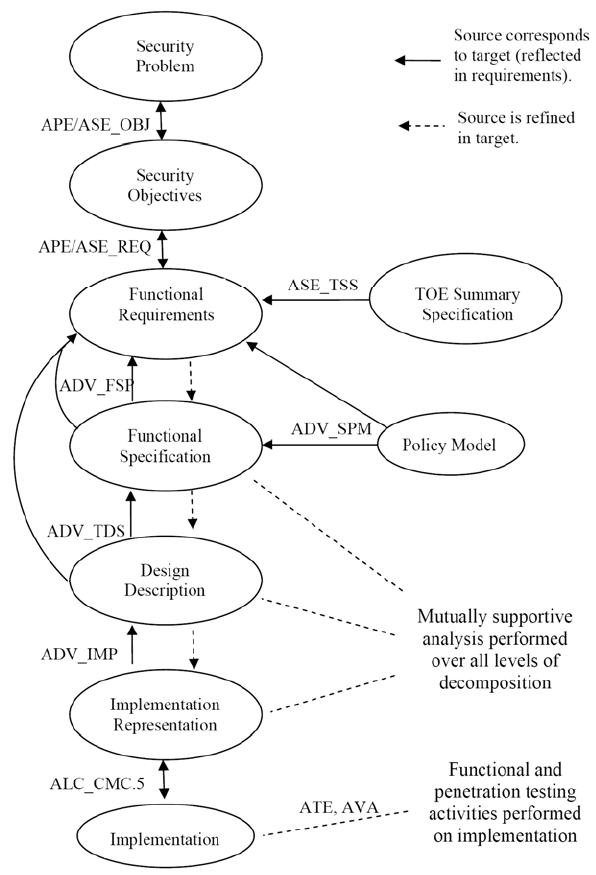
\includegraphics[width=0.45\textwidth, keepaspectratio]{figures/layers.png}
\end{wrapfigure}
\section{Értékelés}

Összességében úgy gondolom, hogy az érintett követelmények, és az azokra adott javaslatok bevezetése
mind a termékfejlesztés hatékonyságát, mind a biztosított minőséget, mind a termék biztonságát
növelte.


Tapasztalataim szerint azáltal, hogy a Common Criteria is rávilágít egyes anomáliákra, indokoltabbá
válhat ezeknek az anomáliáknak a felszámolása, az esetleges \emph{workaround}-ok kevésbé
tekinthetőek elfogadhatónak. Ez a pszichológiai hatás számomra váratlan volt, de mindenképpen
pozitívumként tekintek rá.

\section{Továbbfejlesztési lehetőségek}
Tekintve, hogy a szakdolgozat a Common Criteria követelményeinek csupán egy kis, valódi részhalmazát
dolgozta fel, például az egyik leglényegesebb, és időigényesebb, (biztonsági) funkcionalitással
foglalkozó osztályai nem kerültek tárgyalásra, így nem került említésre a Common Criteria egyik
lényeges funkciója, amely segít azt belátni, hogy az alacsonyabb szintű implementáció megoldást
nyújt a magas szinten lévő biztonsági problémára.
Úgy gondolom, hogy a szakdolgozatban elkezdett elemzés könnyedén folytatható a további osztályok
lefedésével, és a modernizálás utáni (amikor már a fejlesztők megszokták és elfogadták
a változtatásokat) tapasztalatok összegyűjtésével.

\chapter{Továbbfejlesztési lehetőségek}
\todo[inline]{A Common Criteria valódi eszközeiről lehet itt írni.}

%----------------------------------------------------------------------------
\chapter*{Köszönetnyilvánítás}\addcontentsline{toc}{chapter}{Köszönetnyilvánítás}
%----------------------------------------------------------------------------

Szeretnék köszönetet mondani konzulenseimnek, \mbox{Dr. Félegyházi Márknak} és \mbox{Budai
Lászlónak} segítségükért és végtelen türelmükért, \mbox{Badics Alexnek} a segítségéért a Common
Criteria értelmezésében, és tapasztalatainak megosztásáért.
Köszönettel tartozom még a \emph{syslog-ng} fejlesztőinek, hogy a fejlődés érdekében szembenéztek
a múltban hozott döntéseikkel.


%\listoffigures\addcontentsline{toc}{chapter}{Ábrák jegyzéke}
%\listoftables\addcontentsline{toc}{chapter}{Táblázatok jegyzéke}

\bibliography{mybib}
\addcontentsline{toc}{chapter}{Irodalomjegyzék}
\bibliographystyle{plain}

%----------------------------------------------------------------------------
\appendix
%----------------------------------------------------------------------------
\chapter*{Függelék}\addcontentsline{toc}{chapter}{Függelék}
\setcounter{chapter}{6}  % a fofejezet-szamlalo az angol ABC 6. betuje (F) lesz
\setcounter{equation}{0} % a fofejezet-szamlalo az angol ABC 6. betuje (F) lesz
\numberwithin{equation}{section}
\numberwithin{figure}{section}
\numberwithin{lstlisting}{section}
%\numberwithin{tabular}{section}

%----------------------------------------------------------------------------
\section{A TeXnicCenter felülete}
%----------------------------------------------------------------------------
\begin{figure}[!ht]
\centering
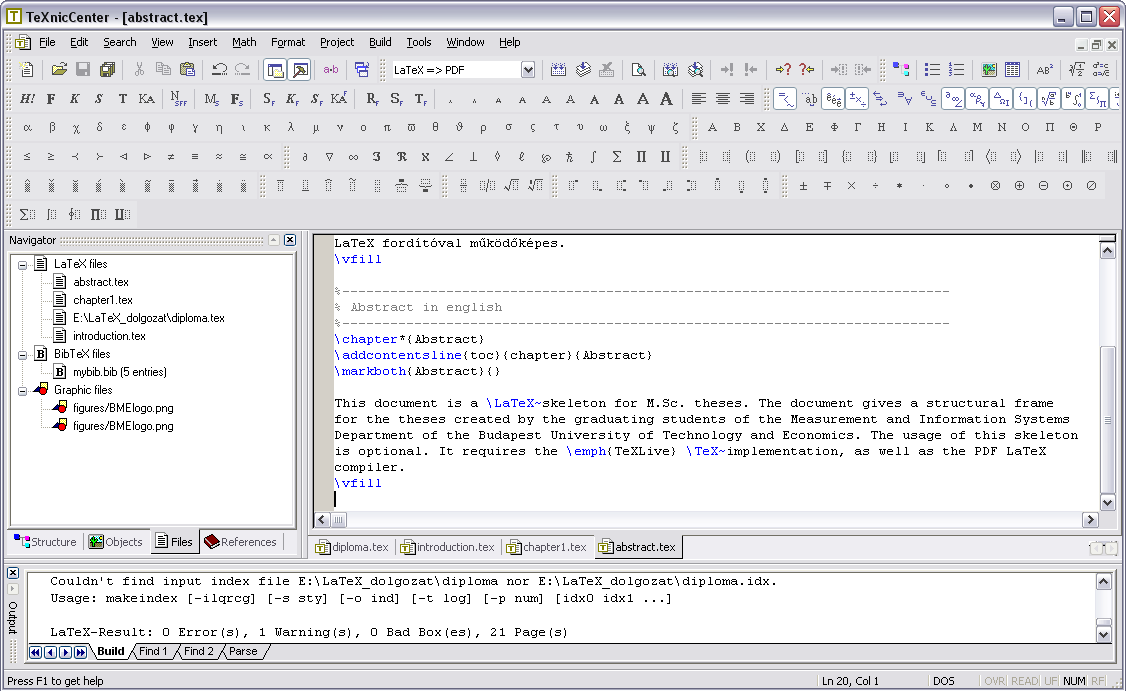
\includegraphics[width=150mm, keepaspectratio]{figures/TeXnicCenter.png}
\caption{A TeXnicCenter Windows alapú \LaTeX-szerkesztõ.} 
\end{figure}

%----------------------------------------------------------------------------
\clearpage\section{Válasz az ,,Élet, a világmindenség, meg minden'' kérdésére}
%----------------------------------------------------------------------------
A Pitagorasz-tételbõl levezetve
\begin{align}
c^2=a^2+b^2=42.
\end{align}
A Faraday-indukciós törvénybõl levezetve
\begin{align}
\rot E=-\frac{dB}{dt}\hspace{1cm}\longrightarrow \hspace{1cm}
U_i=\oint\limits_\mathbf{L}{\mathbf{E}\mathbf{dl}}=-\frac{d}{dt}\int\limits_A{\mathbf{B}\mathbf{da}}=42.
\end{align}







\label{page:last}
\end{document}
